\documentclass[12pt]{amsart}
\usepackage{amsfonts,latexsym,amsthm,amssymb,amsmath,amscd,euscript,tikz}
\usepackage{framed}
\usepackage{fullpage}
\usepackage{comment}
\usepackage{tikz}
\usepackage{bm}
\usepackage{enumerate}
\usepackage{dsfont}
\usepackage{hyperref}
\usetikzlibrary{patterns}
\usepackage{subfig}
\usepackage{float}
\usepackage{listings}
\usepackage{tcolorbox}
% \usepackage[cache=false]{minted}

\lstset{
  basicstyle=\footnotesize,
  xleftmargin=.2\textwidth, xrightmargin=.2\textwidth
}

\usetikzlibrary{decorations.markings,decorations.pathmorphing}
\usepackage{tikz-cd}
\usepackage{enumitem}
\usepackage{hyperref}
    \hypersetup{colorlinks=true,citecolor=blue,urlcolor =blue,linkbordercolor={1 0 0}}

\newenvironment{statement}[1]{\smallskip\noindent\color[rgb]{0.0,0.0,0.0} {\bf #1.}}{}
\newenvironment{solution}[1]{\vspace{5mm}\smallskip\noindent\color[rgb]{0.0,0.0,0.75} {\bf #1.}}{}
\allowdisplaybreaks[1]

% You can define new commands to make your life easier.
\newcommand{\BR}{\mathbb R}
\newcommand{\BC}{\mathbb C}
\newcommand{\BF}{\mathbb F}
\newcommand{\BQ}{\mathbb Q}
\newcommand{\BZ}{\mathbb Z}
\newcommand{\BN}{\mathbb N}
\newcommand{\BE}{\mathbb E}
\newcommand{\Grass}{\text{G}}
\newcommand{\Rain}{\text{R}}
\newcommand{\Sprinkler}{\text{S}}
\newcommand{\True}{\text{True}}
\newcommand{\False}{\text{False}}

\newcommand{\CU}{\mathcal{U}}
\newcommand{\CO}{\mathcal{O}}
\newcommand{\CC}{\mathcal{C}}
\newcommand{\Ob}{\operatorname{Ob}}
\newcommand{\Mor}{\operatorname{Mor}}


% We can even define a new command for \newcommand!
\newcommand{\C}{\mathbb{C}}
\newcommand{\F}{\mathbb{F}}
\newcommand{\Q}{\mathbb{Q}}
\newcommand{\Z}{\mathbb{Z}}
\newcommand{\R}{\mathbb{R}}
\newcommand{\N}{\mathbb{N}}
\newcommand{\bP}{\mathbb{P}}

\newcommand{\Hom}{\operatorname{Hom}}
\newcommand{\End}{\operatorname{End}}
\newcommand{\ch}{\operatorname{char}}
\newcommand{\image}{\operatorname{im}}
\newcommand{\kernel}{\operatorname{ker}}
\newcommand{\rank}{\operatorname{rank}}
\newcommand{\sym}{\operatorname{Sym}}
\newcommand{\im}{\operatorname{im}}
\newcommand{\lcm}{\operatorname{lcm}}
\newcommand{\Res}{\operatorname{Res}}

\newcommand{\Pois}{\text{Pois}}
\newcommand{\ex}{\text{exp}}
\newcommand{\Var}{\text{Var}}
\newcommand{\Binom}{\text{Binom}}
\newcommand{\btheta}{\bm\theta}
\newcommand{\bT}{\bm T}
\newcommand{\E}{\mathbb{E}}
\newcommand{\I}{\mathbb{I}}
\newcommand{\BP}{\mathbb{P}}
\newcommand{\x}{\bm x}
\newcommand{\y}{\bm y}
\newcommand{\z}{\bm z}
\newcommand{\bmT}{\bm T}
\newcommand{\bmX}{\bm X}
\newcommand{\bmY}{\bm Y}
\newcommand{\bmZ}{\bm Z}
\newcommand{\br}{\bm r}
\newcommand{\bI}{\bm I}
\newcommand{\1}{\mathds{1}}
\newcommand{\Score}{\operatorname{Score}}



% If you want a new function, use operatorname to define that function (don't use \text)

\renewcommand{\baselinestretch}{1.25}


\usepackage{dcolumn}
\usepackage{booktabs}
\usepackage{tikz}
\usetikzlibrary{positioning,shapes,arrows}

\newcolumntype{M}[1]{D{.}{.}{1.#1}}


% If you want a new function, use operatorname to define that function (don't use \text)

\renewcommand{\baselinestretch}{1.25}


\title{CS 182 Fall 2022, Problem Set 3}

\begin{document}
\tcbset{colback=blue!5!white}

\maketitle

\vspace*{-0.25in}
\centerline{Due: November 7, 2022 11:59pm}


\begin{center}
\end{center}
\vspace*{0.15in}


\noindent This problem set covers Lectures 10 through 14. The topics include AI game playing, Stackelberg security games, social choice, Bayesian networks, and hidden Markov models.
\vspace*{0.35in}

\begin{statement}{1} \emph{Stackelberg Security Game.} (10 points) Consider a 2-player game in normal form. Let $(x_1,x_2)$ be a (possibly mixed) Nash equilibrium. Show that if $(x_1^\star,s_2)$ is a strong Stackelberg equilibrium (where player 1 is the leader) then $u_1(x_1^\star,s_2)\geq u_1(x_1,x_2)$.
\end{statement}

\newpage

\begin{statement}{2} \textit{Social Choice.} (20 Points) 
Recall that a voting rule is Condorcet consistent if the rule selects an alternative that is a Condorcet winner whenever there exists a Condorcet winner in the given preference profile. As in class we denote the set of voters by $N=\{1,\ldots,n\}$ and the set of alternatives by $A$, where $|A|=m$.

\begin{enumerate}
    \item (10 points) The minimax voting rule (not to be confused with the minimax algorithm) picks an alternative that minimizes the maximum number of voters by which another alternative beats this one, i.e., 
    \[ \operatornamewithlimits{argmin}_{x\in A}\max_{y\in A\setminus\{x\}} \operatorname{Score}(y, x),\]
    where $\operatorname{Score}(y, x) = \sum_{i=1}^n \1[y\succ_i x]$ counts the number of voters who prefer $y$ over $x$, with $\succ_i$ denoting preference according to the ranking of voter $i$. For example, in the profile on slide 5 of Lecture 11, $\operatorname{Score}(b,c)=4$, as there are 4 voters who prefer $b$ to $c$. The minimax rule would choose $b$, as $\max_{y\in A\setminus\{b\}} \operatorname{Score}(y, b)=\operatorname{Score}(a,b)=2$.\\ 
    Show that the minimax rule is Condorcet consistent. You may assume that the number of voters $n$ is odd.
    \begin{tcolorbox}
        First, suppose there is a condorcet winner, $x^*$, in the profile. This means that $x^*$ beats all other alternates in a head-to-head 
        plurality vote, so 
        \begin{align*}
            \Score(y, x*) < \Score(x^*, y)
        \end{align*}
        for all $y\in A\setminus\{ x^* \}$
    \end{tcolorbox}
    \item (10 points) A \textit{positional scoring rule} using a score vector $(s_1, \ldots, s_m)$, where $s_1 \geq \cdots \geq s_m$, is one that determines a winner by picking an alternative with maximum score, where scores are determined as follows:
    \begin{itemize}
        \item Each voter $i$ gives $s_j$ points to the alternative that is the $j$th highest on their ranking (e.g., the highest alternative in $\sigma_i$ receives $s_1$ points and the lowest alternative $\sigma_i$ receives $s_m$ points).
        \item Each alternative's score is the sum of the points given over all voters.
    \end{itemize}
    Answer the following questions about positional scoring rules.
    \begin{enumerate}
        \item (4 points) Explain why both Plurality voting and Borda voting are examples of positional scoring rules.
        \item (6 points) Under the assumption that $s_1>s_2>\cdots >s_m$, prove that no positional scoring rule is Condorcet consistent.\\
        \textbf{Hint}: Construct a preference profile with three alternatives and a smallish number of voters such that there is a Condorcet winner but any positional scoring rule with $s_1>s_2>s_3$ would select a different alternative. 
    \end{enumerate}
\end{enumerate}
\end{statement}

\newpage

\begin{statement}{3}
\emph{Bayesian Networks.} (10 points) Consider the following Bayes net:

\newcommand{\vara}{Sprinkler}
\newcommand{\varb}{Grass wet}
\newcommand{\varc}{Rain}
\begin{center}
\begin{tikzpicture}[
  node distance=1cm and 0cm,
  mynode/.style={draw,ellipse,text width=2cm,align=center}
]
\node[mynode] (sp) {\vara};
\node[mynode,below right=of sp] (gw) {\varb};
\node[mynode,above right=of gw] (ra) {\varc};
\path (ra) edge[-latex] (sp)
(sp) edge[-latex] (gw) 
(gw) edge[latex-] (ra);
\node[left=0.5cm of sp]
{
\begin{tabular}{cM{2}M{2}}
\toprule
& \multicolumn{2}{c}{\vara} \\
Rain & \multicolumn{1}{c}{T} & \multicolumn{1}{c}{F} \\
\cmidrule(r){1-1}\cmidrule(l){2-3}
F & 0.4 & 0.6 \\
T & 0.1 & 0.9 \\
\bottomrule
\end{tabular}
};
\node[right=0.5cm of ra]
{
\begin{tabular}{M{1}M{1}}
\toprule
\multicolumn{2}{c}{\varc} \\
\multicolumn{1}{c}{T} & \multicolumn{1}{c}{F} \\
\cmidrule{1-2}
0.2 & 0.8 \\
\bottomrule
\end{tabular}
};
\node[below=0.5cm of gw]
{
\begin{tabular}{ccM{2}M{2}}
\toprule
& & \multicolumn{2}{c}{\varb} \\
\multicolumn{1}{l}{\vara} & \multicolumn{1}{l}{\varc} & \multicolumn{1}{c}{T} & \multicolumn{1}{c}{F} \\
\cmidrule(r){1-2}\cmidrule(l){3-4}
F & F & 0.1 & 0.9 \\
F & T & 0.2 & 0.8 \\
T & F & 0.3 & 0.7 \\
T & T & 0.4 & 0.6 \\
\bottomrule
\end{tabular}
};

\end{tikzpicture}
\end{center}
    In each table, the value of the conditioned variables are presented on the leftmost columns.
    \begin{enumerate}
        \item (3 points) What is $\mathbb{P}(\text{Grass wet}=\text{True}\mid \text{Rain}=\text{False})$?
        \begin{tcolorbox}
            By the definition of conditional probability,
            \begin{align*}
                 \bP(\text{Grass wet} = \text{True}\mid \text{Rain}=\text{False}) &= \frac{\bP(\text{Grass wet} = \text{True}\cap \text{Rain}=\text{False})}{\bP(\text{Rain}=\text{False})}
            \end{align*}
            The denominator is given, but the numerator can be found using LOTP
            \begin{align*}
                \bP(\Grass \cap \Rain^c) = \bP(\Grass\cap \Rain^c\cap \Sprinkler) + \bP(\Grass\cap\Rain^c \cap \Sprinkler^c)
            \end{align*}
            where G, R, and S are used as shorthand for Grass = True,... and so on and G$^c$, R$^c$, and S$^c$ are shorthand for 
            Grass = False... and so on. \\ 
            By the chain rule, we have 
            \begin{align*}
                \bP(\Grass\cap\Sprinkler\cap\Rain^c) &= \bP(\Grass\mid \Rain^c\cap \Sprinkler)*\bP(\Sprinkler\mid \Rain^c)*\bP(\Rain^c)\\ 
                &= 0.3*0.4*0.8\\ 
                &= 0.096
            \end{align*}
            Similarly, we have
            \begin{align*}
                \bP(\Grass\cap\Sprinkler^c\cap\Rain^c) &= \bP(\Grass\mid \Rain^c\cap \Sprinkler^c)*\bP(\Sprinkler^c\mid \Rain^c)*\bP(\Rain^c)\\ 
                &= 0.1*0.6*0.8\\
                &= 0.048
            \end{align*}
            Thus, 
            \begin{align*}
                \bP(\Grass\mid \Rain^c) &= \frac{0.096 + 0.048}{0.8}\\ 
                &= 0.18
            \end{align*}
        \end{tcolorbox}
        \item (3 points) What is $\mathbb{P}(\text{Grass wet}=\text{True})$?
        \begin{tcolorbox}
            Using LOTP and the chain rule we get 
            \begin{align*}
                \bP(\Grass) &= \bP(\Grass\cap\Rain\cap\Sprinkler) + \bP(\Grass\cap\Rain^c\cap\Sprinkler) + \bP(\Grass\cap\Rain\cap\Sprinkler^c) + \bP(\Grass\cap\Rain^c\cap\Sprinkler^c)\\ 
                &= \bP(\Grass\mid\Rain\cap\Sprinkler)*\bP(\Sprinkler\mid\Rain)*\bP(\Rain) + \bP(\Grass\mid\Rain^c\cap\Sprinkler)*\bP(\Sprinkler\mid\Rain^c)*\bP(\Rain^c) \\ 
                &+ \bP(\Grass\mid\Rain\cap\Sprinkler^c)*\bP(\Sprinkler^c\mid\Rain)*\bP(\Rain) + \bP(\Grass\mid\Rain^c\cap\Sprinkler^c)*\bP(\Sprinkler^c\mid\Rain^c)*\bP(\Rain^c)\\ 
                &= 0.4*0.1*0.2 + 0.3*0.4*0.8 + 0.2*0.9*0.2 + 0.1*0.6*0.8\\
                &= 0.188
            \end{align*}
        \end{tcolorbox}
        \item (4 points) Suppose we did likelihood weighting on this network, where we observe evidence $Sprinkler=True$.
        What is the weight of a sample \[\bm x = (Rain=True, Sprinkler=True, GrassWet=False)\] obtained from the \textsc{Weighted-Sample} algorithm?\\ 
        \begin{tcolorbox}
            In the algorithm, $\text{Sprinkler} = \True$ is set first without changing $w$. Then, the algorithm sees that $X_i = \Sprinkler$ is an evidence 
            variable and adjusts $w$ \\as $w \gets w*\bP(\text{Sprinkler}=\True\mid \text{parents}(\text{Sprinkler})) = 1 * \bP(\text{Sprinkler} = \True \mid 
            \text{Rain} = \True) = 0.1$
        \end{tcolorbox}
    \end{enumerate}

\end{statement}

\newpage

\begin{statement}{4}
\textit{Hidden Markov Models.} (20 Points) Alice and Bob are living in a house. Bob never leaves the house or checks the weather outside, so he never knows for sure if it is rainy or sunny (assume for simplicity these are the only two weather phenomena).
However, Alice does leave the house, and her mood is determined stochastically by the status of the weather that day.
Bob is able to make inferences about the weather based on Alice's mood when she gets home, so he uses a hidden markov model in which the weather describes the underlying hidden states and Alice's mood are his observed states. He knows that in his city of Markovtown, 
\begin{itemize}
    \item If it is raining today, then it will rain with probability $0.8$ on the next day.
    \item If it is currently sunny, then it will be sunny with probability $0.6$ on the next day.
\end{itemize}
He also knows that Alice's mood depends on the weather in the following process:
\begin{itemize}
    \item If it is raining, then Alice will be in a bad mood with probability $0.7$.
    \item If it is sunny, then Alice will be in a good mood with probability $0.6$.
\end{itemize}
One day, Bob checks the weather channel, so he knows for sure that it rained. He then recorded Alice's mood the next three days (not including the day he checked the weather channel): good, good, bad.
\begin{enumerate}
    \item (10 points) What is the probability that it will be rainy on day $4$?
    \item (10 points) Under Bob's model, what is the most likely sequence of weather states over the three days?
\end{enumerate}
\end{statement}

\newpage

\begin{statement}{5}
\textit{AI Game Playing.} (35 points)\emph{AI Game playing in Ghost. }In this problem, you will solve the game of \textit{Ghost}\footnote{The authors of this problem are unclear whether this is the universal name for this game, but we shall go with it.} using alpha-beta pruning. This game is played with two players, as follows. The first player chooses an English letter, the second player adds another letter to the end of the first player's letter, the first player then adds another letter to the end of that, and so on. The key is that, at any given point in time, the growing string must have the ability to form a word, but the first player who is forced to make the string into a word loses. For example, an example game might play out as follows:
\begin{align*}
    \text{First Player: }& W \quad \textit{// Growing string: ``W"} \\
    \text{Second Player: }& A \quad \textit{// Growing string: ``WA"} \\
    \text{First Player: }& T \quad \textit{// Growing string: ``WAT"} \\
    \text{Second Player: }& E \quad \textit{// Growing string: ``WATE"} \\
    \text{First Player: }& R \quad \textit{// Game ends, ``WATER" forms a word}
\end{align*}
Note that the first player played an $R$ at the end, so since ``WATER" is a word, the first player loses. \\

We have modified the game in the following way: the value of a player's is the reciprocal of the length of the word in the terminal state, flipped with the appropriate sign depending on which player's turn it is.
This has the effect that players aren't merely interested in winning, but they are also interested in winning quickly whenever they can guarantee their victory, and they want to make the game last as long as possible if their opponent can guarantee victory instead,

\noindent
The code file is located in \texttt{pset3.py}. We have included a text file of English words in \texttt{dictionary.txt}. Note that you only have to implement the alpha-beta pruning agent, and not any of the Ghost game details. Our autograder will run your agent against ours and check that your agent wins in all the situations in which it should win. Note that the Gradescope Autograder corresponds to the point values in parts $(1)$, $(2)$, and $(4)$ of this problem.
\textbf{How to tiebreak: For all agents, if several actions result in states with the same value, then we pick the action that is first in our \texttt{get\_actions()} list (e.g. in the Ghost game, this should just be alphabetical order). Additionally, do not make any unnecessary calls to \texttt{get\_actions()} or the autograder will fail the test cases.}
\begin{enumerate}
    \item (5 points) Implement the \texttt{MinimaxAgent}.
    \item (10 points) \texttt{AlphaBetaAgent.} \begin{enumerate}
        \item (5 Points) Paul and Fiona decide to play one final game, in which Paul is attempting to maximize his score, while Fiona attempts to minimize Paul's score. Both Paul and Fiona play optimally, and the game tree is shown in the following figure. Perform the minimax algorithm with alpha-beta pruning to find the alpha and beta values passed to each node when the node is first called. Include an image with the alpha beta values at each node, as well as an indication of which branches are pruned. Assume that the algorithm visits each child from left to right. What are the actions that each player takes?
\vspace{-3mm}
 \begin{figure}[H]
        \centering
        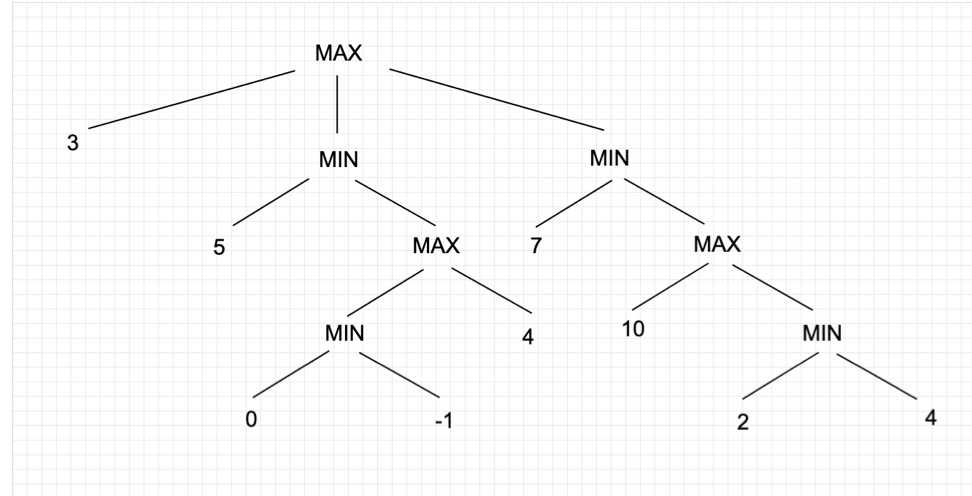
\includegraphics[width=0.5\textwidth]{alpha-beta.png}
        \vspace{-5mm}
        \caption{Game Tree for Problem 1}
\end{figure}
\vspace{-5mm}
        \item (5 Points) Implement the \texttt{AlphaBetaAgent}. You should find that the number of calls to \texttt{getSuccessor} is smaller than before (which would indicate that pruning has improved our search).
    \textbf{You should prune on equality} $\alpha=\beta$ \textbf{in order for the autograder to recognize your submission.}
    \end{enumerate}
    \item (5 points) Recall that the minimax algorithm helps you find the optimal value against an opponent who is also playing optimally. Now suppose that you know that your opponent is not necessarily playing smart; instead, your opponent simply just picks a random letter that is a valid move.
    Describe the strategy that maximizes or minimizes (depending on whether you are the max or the min agent) the expected value of the terminal game state.
    \item (10 points) Implement the agent in part (3) in \texttt{OptimizedAgainstRandomAgent}. You should implement both cases, whether the agent wants to maximize or minimize the terminal value of the game, depending on the agent's index.
    \item (5 points) In \texttt{simulate\_versus\_random}, we compare the performance of the agent from part (4) against a random agent with the performance of a minimax agent against a random agent.
    We take the random agent to be the minimizer.
    We compute the average value that each agent wins over \texttt{k=10000} trials. By about how much does your agent from (4) beat the minimax agent on the initial game state prefixes  [\texttt{beh}, \texttt{feb}, \texttt{gw}]?
    Explain your intuition for why the \texttt{OptimizedAgainstRandomAgent} beats the \texttt{MinimaxAgent} on average against a random agent (there is more than one possible answer to this question).
\end{enumerate}
\end{statement}

\newpage

\begin{statement}{6}
\noindent \textbf{Collaboration, Calibration and References} (5 points).
\begin{enumerate}
    \item With whom did you work on this problem set? What (if any) references and/or resources did you use beyond the course lecture slides and textbook? 
    \item (5 points) Approximately how long did it take you to complete this problem set? Please complete this brief \href{https://forms.gle/S3UGVtR8jDf4gQvN7}{survey} worth 5 points, graded for completion.
\end{enumerate}
\end{statement}


\end{document}

